\section*{Section \ref{S:uncountablesets} Uncountable Sets}

\begin{enumerate}
\item \begin{enumerate}
\item $f:\left( 0, \infty \right) \to \mathbb{R}$ by $f \left( x \right) = \ln x$ for all 
$x \in \left( 0, \infty \right)$.

\item $g: \left( 0, \infty \right) \to \left( a, \infty \right)$ by $g \left( x \right) = x + a$ for all $x \in \left( 0, \infty \right)$.  The function $g$ is a bijection and so 
$\left( 0, \infty \right) \approx \left( a, \infty \right)$.  Then use Part~(a).

\item Let $\mathbb{Z}^* = \left\{ x \in \mathbb{Z} \mid x \geq 0 \right\}$.  Define 
$f : \mathbb{R} \to \left( \mathbb{R} - \left\{ 0 \right\} \right)$ as follows:
\begin{equation} \notag
f \left( x \right) = 
\begin{cases}
x         &\text{if } x \notin \mathbb{Z}^* \\
 %                     &                      \\
x +1        &\text{if } x \in \mathbb{Z}^*.
\end{cases}
\end{equation}
The function $f$ is a bijection and so 
$\mathbb{R} \approx \left( \mathbb{R} - \left\{ 0 \right\} \right)$.


\item $g: \left( \mathbb{R} - \left\{ 0 \right\} \right) \to 
\left( \mathbb{R} - \left\{ a \right\} \right)$ by $g \left( x \right) = x + a$ for all 
$x \in \mathbb{R}$.  The function $g$ is a bijection and so 
$\left( \mathbb{R} - \left\{ 0 \right\} \right) \approx 
\left( \mathbb{R} - \left\{ a \right\} \right)$.

\end{enumerate}

\item Let $\mathbb{H}$ be the set of irrational numbers.  Then 
$\mathbb{R} = \mathbb{Q} \cup \mathbb{H}$ and $\mathbb{Q}$ and $\mathbb{H}$ are disjoint.  So if $\mathbb{H}$ is countable, then by Theorem~\ref{T:unionofcountable}, $\mathbb{R}$ would be countably infinite.  Therefore, $\mathbb{H}$ is uncountable.

\item By Corollary~\ref{C:subsetofcountable}, every subset of a countable set is countable.  So if 
$B$ is countable, then $A$ is countable.

\item By Cantor's Theorem (Theorem~\ref{T:cantor}), $\mathbb{R}$ and 
$\mathcal{P} \left( \mathbb{R} \right)$ do not have the same cardinality.

\item We use an argument similar to Cantor's diagonal argument to prove that the set $C$   of all infinite sequences, each of whose entries is the digit 0 or the digit 1, is uncountable.

Suppose that there is a function $f: \N \to C$ that is an injection.  We will show that 
$f$ cannot be a surjection by showing that there exists an element in 
$C$ that cannot be in the range of $f$.  We write the images of the elements of 
$\N$ as follows:

\[
\begin{aligned}
f \left( 1 \right) &= \left(a_{1 1}, a_{1 2}, a_{1 3}, a_{1 4}, a_{1 5}, \ldots \right) \\
f \left( 2 \right) &= \left(a_{2 1}, a_{2 2}, a_{2 3}, a_{2 4}, a_{2 5}, \ldots \right) \\
f \left( 3 \right) &= \left(a_{3 1}, a_{3 2}, a_{3 3}, a_{3 4}, a_{3 5}, \ldots \right) \\
f \left( 4 \right) &= \left(a_{4 1}, a_{4 2}, a_{4 3}, a_{4 4}, a_{4 5}, \ldots \right) \\
f \left( 5 \right) &= \left(a_{5 1}, a_{5 2}, a_{5 3}, a_{5 4}, a_{5 5}, \ldots \right) \\
                   & \vdots \\
f \left( n \right) &= \left(a_{n 1}, a_{n 2}, a_{n 3}, a_{n 4}, a_{n 5}, \ldots \right) \\
                   & \vdots \\
\end{aligned}
\]

Notice the use of the double subscripts. The number $a_{i j}$ is the $j${th} term of the infinite sequence $f \left( i \right)$, and $a_{i j}$ must be 0 or 1.

We will now construct an infinite sequence $b = \left(b_1, b_2, b_3, b_4, b_5, \ldots \right)$ in $S$ that is not in this list.  

Start with $a_{1 1}$ in $f \left( 1 \right)$.  We choose $b_1$ so that $b_1 \ne a_{1 1}$.  This can be done as follows:  If $a_{1 1} = 0$, then choose $b_1 = 1$, and if $a_{1 1} = 1$, then choose $b_1 = 0$.

We then repeat this process with $a_{2 2}$, $a_{3 3}$, 
$a_{4 4}$, $a_{5 5}$, and so on.  That is, we choose $b_2$ so that $b_2 \ne a_{2 2}$, 
choose $b_3$ so that $b_3 \ne a_{3 3}$, and so on.

We then let $b = \left(b_1, b_2, b_3, b_4, b_5, \ldots \right)$  for each $k \in \N$,

\begin{equation} \notag
b_k = 
\begin{cases}
1         &\text{if $a_{k k} = 0$} \\
0         &\text{if $a_{k k} = 1$}
\end{cases}
\end{equation}

Now, for each $n \in \N$, $b \ne f \left( n \right)$ since $b$ and $f \left( n \right)$ differ in the $n${th} term of their sequences.

This proves that any injective function from $\N$ to $C$ cannot be surjection and hence, there is no bijection from $\mathbb{N}$ to $\left( 0, 1 \right)$.  Therefore, 
$S$ is not countably infinite and hence must be an uncountable set.

\item \begin{enumerate}
\item $f: \left( 0, 1 \right) \to \left[ 0, 1 \right]$ by $f \left( x \right) = x$ for all 
$x \in \left( 0, 1 \right)$.

\item $h: \left[ 0, 1 \right] \to \left( -1, 2 \right)$ by $h \left( x \right) = x$ for all 
$x \in \left[ 0, 1 \right]$.

\item Since $\left( -1, 2 \right) \approx \left( 0, 1 \right)$, there exists a bijection 
$k: \left( -1, 2 \right) \to \left( 0, 1 \right)$.  Hence, 
$k \circ h : \left[0, 1 \right] \to  \left( 0, 1 \right)$ is a bijection.

\item Parts~(a) and~(c) and the Cantor-Schr\"{o}der-Bernstein Theorem imply that 
$\left[0, 1 \right] \approx \left( 0, 1 \right)$.
\end{enumerate}

\item Define $f: \left[ a, b \right] \to \left[ 0, 1 \right]$ by 
$f \left( x \right) = \dfrac{x - a}{b - a}$ for all $x \in \left[ a, b \right]$.  The function 
$f$ is a bijection and hence $\left[ a, b \right] \approx \left[ 0, 1 \right]$.


\item Let $F$ be the set of all finite subsets of $\N$.  We will use the Cantor-Schr\"{o}der-Bernstein Theorem to prove that $F$ is countably infinite.

\newpar
We first define $g: \N \to F$ as follows:  For each $m \in \N$,  $g(m) = \{ m \}$.  It is clear that the function $g$ is an injection.

\newpar
We now let $p_1, p_2, p_3, \ldots, p_k, \ldots$ be the ordered list of prime numbers in ascending order, so that $p_1 < p_2 < \cdots < p_n < \cdots$.  We then define $f: F \to \N$ as follows:

\begin{list}{}
\item If $A \in F$, we write $A = \left\{ a_1, a_2, \ldots, a_m \right\}$ with $a_1 < a_2 < \cdots < a_m$ and define $f(A)$ as follows:
\[
f(A) = p_1^{a_1} p_2^{a_2} \cdots p_m^{a_m}.
\]
\end{list}
We will use the Fundamental Theorem of Arithmetic to prove that $f$ is an injection.  So we let $A, B \in F$ and write
\[
A = \left\{ a_1, a_2, \ldots, a_m \right\} \quad \text{and} \quad B = \left\{ b_1, b_2, \ldots, b_n \right\}.
\]
\setcounter{equation}{0}
So if $f(A) = f(B)$, then
\begin{equation}
p_1^{a_1} p_2^{a_2} \cdots p_m^{a_m} = p_1^{b_1} p_2^{b_2} \cdots p_n^{b_n}.
\end{equation}
As guaranteed by the Fundamental Theorem of Arithmetic, each natural number has a unique prime factorization, and so the prime factorizations in equation~(1) imply that $m = n$ and for each $j$ with $1 \leq j \leq m$, 
$a_j = b_j$.  This in turn implies that the sets $A$ and $B$ have precisely the same elements and so 
$A = B$.  This proves that if $f(A) = f(B)$, then $A = B$ and so the function $f$ is an injection.

\newpar
We now have an injection $g:\N \to F$ and an injection $f:F \to \N$.  Hence, by the 
Cantor-Schr\"{o}der-Bernstein Theorem, $\text{card}(\N) = \text{card}(F)$ and this proves that the set of all finite subsets of $\N$ is countably infinite.





\item \begin{enumerate}
\item The function $f$ defined as follows is an injection.
\[
f\x \Q^c \to \R \quad \text{by} \quad f(x) = x, \text{ for each } x \in \Q^c.
\]

\item If $a \in \R$ and $a = A.a_1 a_2 a_3 a_4 \cdots a_n \cdots$, where $A$ is an integer and the decimal part $( 0.a_1 a_2 a_3 a_4 \cdots )$ is in normalized form, then the real number
\[
A.a_1 0 a_2 1 1 a_3 0 0 0 a_4 1 1 1 1 a_5 0 0 0 0 0 a_6 1 1 1 1 1 1 \cdots 
\]
has an infinite nonrepeating decimal expansion, and hence, it is an irrational number.

\item Define $g\x \R \to \Q^c$ as follows:  If $a \in \R$ and $a = A.a_1 a_2 a_3 a_4 \cdots a_n \cdots$, where $A$ is an integer and the decimal part $( 0.a_1 a_2 a_3 a_4 \cdots )$ is in normalized form, then 
\[
g(a) = A.a_1 0 a_2 1 1 a_3 0 0 0 a_4 1 1 1 1 a_5 0 0 0 0 0 a_6 1 1 1 1 1 1 \cdots \,.
\]
The decimal part of $g(a)$ is in normalized form.  This can be used to prove that $g$ is an injection since two decimal numbers in normalized form are equal if and only if they have identical digits in each decimal position.

\item We can now use the Cantor-Schr\"{o}der-Bernstein Theorem to conclude that $\R$ has the same cardinality as $\Q^c$.
\end{enumerate}



\item \begin{enumerate}
\item \begin{multicols}{2}
$f ( 0.3, 0.625 ) = 0.3602505$ 

$f \!\left( \dfrac{1}{3}, \dfrac{1}{4} \right) = 0.3235303030 \cdots$

$f \!\left( \dfrac{1}{6}, \dfrac{5}{6} \right) = 0.1863636363 \cdots$
\end{multicols}

\item $f(0.24, 0.35) = 0.2345$

\item $f \!\left( \dfrac{1}{3}, \dfrac{1}{3} \right) = \dfrac{1}{3}$

\item There is no $(x, y) \in S$ such that $f(x, y) = \dfrac{1}{2}$.

\item The result in Part~(d) shows that $f$ is not a surjection.  Since the decimal expansions are all in normalized form, if $(a, b) \in S$ and $(c, d) \in S$ with $f(a, b) = f(c, d)$, then the normalized forms of $f(a, b)$ and $f(c, d)$ are identical.  This implies that the normalized form of $a$ and $c$ are identical and the normalized forms of $b$ and $d$ are identical.  Hence, 
$a = c$ and $b = d$ and so, $(a, b) = (c, d)$.  Therefore, $f$ is an injection.

\item The function $f\x S \to J$ in Part~(e) is an injection.  We can also define 
$g\x J \to S$ by $g(a) = (a, 0.5)$ for each $a \in J$.  This function is also an injection and hence, bt the Cantor-Schr\"{o}der-Bernstein Theorem, \linebreak
$S \approx J$.  This means that the cardinality of the open unit square $S$ is equal to $\boldsymbol{c}$.
\end{enumerate}
\end{enumerate}


\subsection*{Explorations and Activities}
\setcounter{oldenumi}{\theenumi}
\begin{enumerate} \setcounter{enumi}{\theoldenumi}
\item \begin{enumerate}
\item Let $f: \left[ 0, 1 \right] \to \left[ 0, 1 \right)$ by
\begin{equation} \notag
f \left( x \right) = 
\begin{cases}
\dfrac{1}{n+1}         &\text{if $x=\dfrac{1}{n}$ for some $n \in \mathbb{N}$} \\
 %                     &                      \\
x        &\text{otherwise}
\end{cases}
\end{equation}
\begin{enumerate}
\item 
$f \left( 0 \right) = 0$,
$f \left( 1 \right) = \dfrac{1}{2}$, 
$f \left( \dfrac{1}{2} \right) = \dfrac{1}{3}$, 
$f \left( \dfrac{1}{3} \right) = \dfrac{1}{4}$, 
$f \left( \dfrac{1}{4} \right) = \dfrac{1}{5}$,
$f \left( \dfrac{1}{5} \right) = \dfrac{1}{6}$.

\item The graph below shows some of the graph of the function $f$.  The points marked with a small square on the line $y = x$ indicate the points that have been removed from this line.  They have been replaced by the points marked with a small circle.  The graph shows 6 points that have been removed and the 6 points that have replaced them.  The process continues, but this is not shown on the graph.
%
\begin{center}
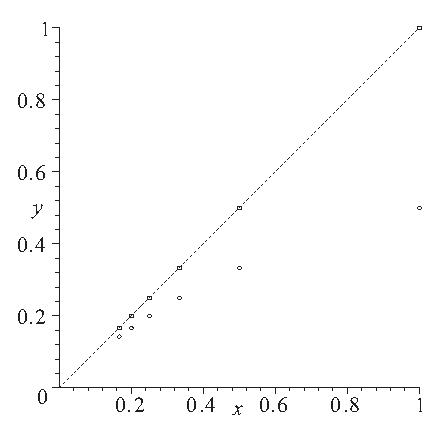
\includegraphics{figps-sec93-1.eps}
\end{center}
%
\item From the graph, we see that function $f$ is an injection.  We also see that the range of 
$f$ is the interval $\left[ 0, 1 \right)$, and hence, $f$ is a surjection.  

\item Since $f$ is a bijection, we conclude that $\left[0, 1 \right] \approx \left[ 0, 1 \right)$.
\end{enumerate}

\item Let $g: \left[ 0, 1 \right) \to \left( 0, 1 \right)$ by
\begin{equation} \notag
g \left( x \right) = 
\begin{cases}
\dfrac{1}{2}           &\text{if $x=0$} \\
%                      &                      \\
\dfrac{1}{n+1}         &\text{if $x=\dfrac{1}{n}$ for some $n \in \mathbb{N}$} \\
%                      &                      \\
x        &\text{otherwise}
\end{cases}
\end{equation}
%
\begin{enumerate}
\item The following graph shows some of the graph of the function $g$.  The points marked with a small square on the line $y = x$ indicate the points that have been removed from this line.  They have been replaced by the points marked with a small circle.  The graph shows 6 points that have been removed and the 6 points that have replaced them.  The process continues, but this is not shown on the graph.  Notice that the point $\left( 0, \dfrac{1}{2} \right)$ has been added, and there is no point on the graph with $x = 1$ since 1 is not in the domain of $g$.

\begin{center}
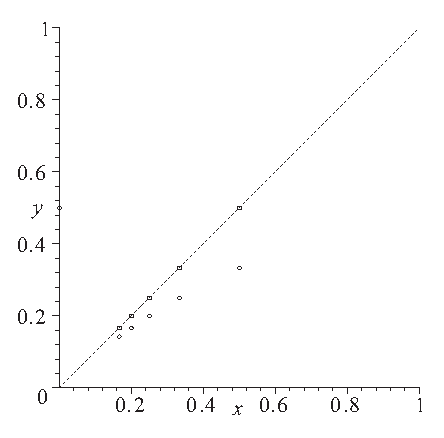
\includegraphics{figps-sec93-2.eps}
\end{center}
%
\item From the graph, we see that function $g$ is an injection.  We also see that the range of 
$g$ is the open interval $\left( 0, 1 \right)$, and hence, $g$ is a surjection.  

\item Since $g$ is a bijection, we conclude that $\left[0, 1 \right) \approx \left( 0, 1 \right)$.
\end{enumerate}

\item Part~(1) and Part~(2) show that the intervals $\left[0, 1 \right]$, $\left[0, 1 \right)$, and $\left(0, 1 \right)$ are all equivalent.  Therefore, each of the intervals is uncountable and has cardinality $\boldsymbol{c}$.


\end{enumerate}


\end{enumerate}

\hbreak
\endinput
